\subsection{Multi modal similarity}
We now take a look at multimodal similarity. Here we have used image A and image A inverted, that is, the intensities have been multiplied by -1. The results can be seen in \autoref{multiModal}.

\begin{figure}
	\centering
	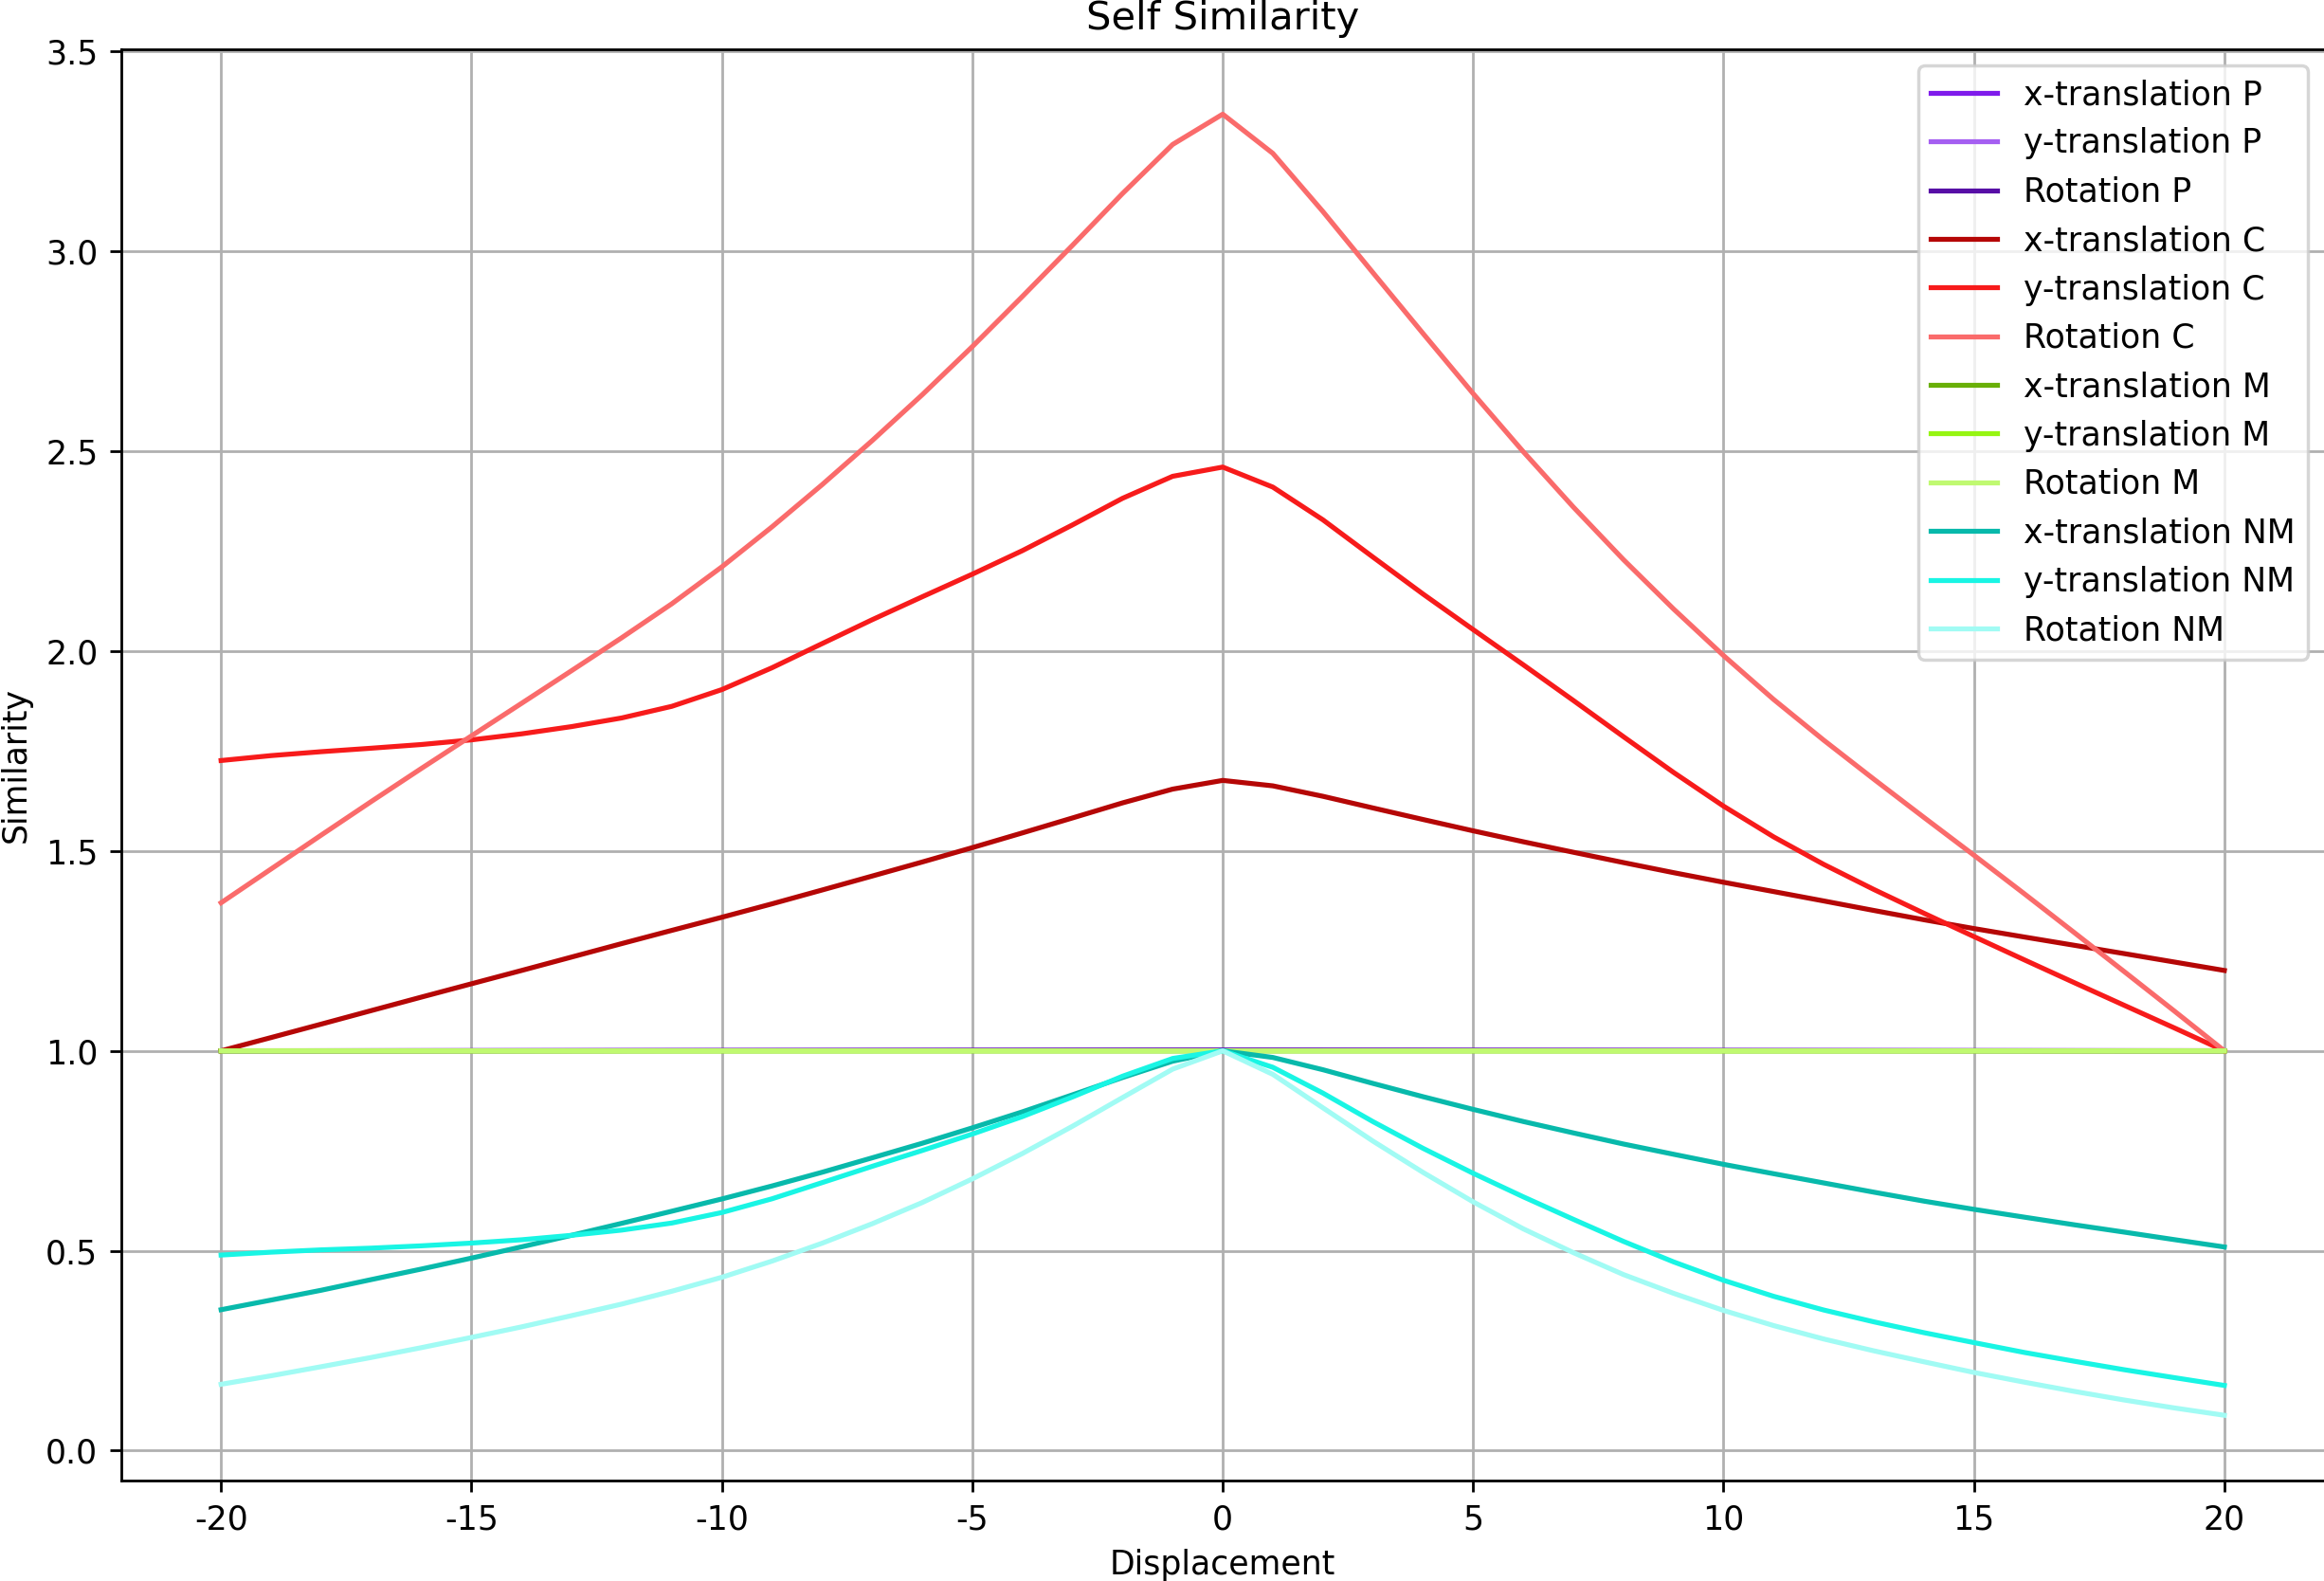
\includegraphics[width=0.8\linewidth]{Materials/multiModalSimilarity}
	\caption{Multi modal similarity results normalized such that all optima touch 1.0. Both images have been blurred by a Gaussian kernel with sigma being 1. Translation displacement is measured in pixels and rotation displacement is measured in degrees. P = P-norm with P being 2, C = normalized cross correlation, M = mutual information, NM = normalized mutual information.}
	\label{multiModal}
\end{figure}
Although it is hard to see, we have that the P-norm is slightly above 1.0 except when the displacements are greatest where it touches 1.0, and we have MI is slightly below 1.0 except when we have 0 displacement where it touches 1.0. We note that NCC now finds the optimal similarities when the displacements are greatest and the smallest similarity when the displacements are 0 as we have normalized the similarities such that the optima touches 1.0. This means NCC is not invariant to intensity changes, and thus is not suitable as a similarity measure for multi modal images. The same is the case for P-norm which also has its optima where the displacement is greatest. We see that  MI behaves correctly and thus is invariant to intensity changes, however, MI become extremely flat, and so its gradients are almost 0. This would make it very hard to optimize the similarity measure with a gradient based method, but it is smooth. Lastly we have NMI which also shows invariance to intensity changes and, of the correctly behaving similarity measures, shows the greatest sensitivity to the displacements. This makes the gradients bigger and thus the function easier to optimize. We also see the curves being more smooth than during self similarity.\\
The reason for P-norm and NCC not being invariant to these intensity changes is they both rely on intensities to compute the similarity, and thus, when we invert one of the images we get negative values as part of the similarity measures, which seemingly flips everything around the x-axis. As MI and NMI works on the distribution of the intensities, and not the intensities themselves, it does not matter if the values have been inverted, it only matter whether we observe as many inverted values as non-inverted values, i.e. that the distribution of pixels are the same in the two images.